\chapter{Tabellen und Abbildungen}
\section{Tabellen}
Die beiden wichtigsten Regeln für die Erstellung schöner Tabellen lauten:
\begin{enumerate}
 \item Nie vertikale Linien benutzen.
 \item Nie doppelte Linien benutzen.
\end{enumerate}
Das Paket \code{booktabs} vereinfacht. Zusätzlich in Tab.\,\ref{tab:tabelle} \code{threeparttable} verwendet. Dieses Paket erlaubt die Benutzung von Fußnoten und Anmerkungen in Tabellen. Außerdem zeigt das Beispiel die Verwendung des von \code{siunitx} gelieferten Spaltenstils. Mit diesem können Unsicherheiten bequem automatisch formatiert und Werte gerundet werden. 
\begin{table}[htb]
    \centering
    \caption[Verwendung von \texttt{table}]{Man beachte, dass $E_\text{tot,1}$ und $E_\text{tot,2}$ das selbe Ergebnis liefern, obwohl sie im Quelltext unterschiedlich formatiert wurden.}
    \label{tab:tabelle}
  \begin{threeparttable}
    \sisetup{
    table-align-text-post = false
    }
\begin{tabular}{
S[table-format = 2.2]
c
S[table-format = 2.1(1),separate-uncertainty = true]
S[table-format = 2.1(1),separate-uncertainty = true]
S[table-format = 4.2(1),separate-uncertainty = false]
S[table-format = 3.1,round-mode=places,round-precision=1]
}
\toprule
{$N_{\text{particles,min}}$}  & 
{Hier} &
{$E_\text{tot,1}$ / \si{\giga \electronvolt}} &
{$E_\text{tot,2}$ / \si{\GeV}} &
{$F$ / \si{\newton}} & 
{${N'}$} \\
\midrule
   10.14\tnote{a}     &       steht       &    18.3(2)        &   18.3+-0.2   &   4018.95(3)  &   282.25 \\
   11.54              &       nur         &    18.4(3)        &   18.4+-0.3   &   3991.32(4)  &   246.45 \\
   12.34              &       zentrierter &    10.4(2)        &   10.4+-0.2   &   3981.19(2)  &   230.78 \\
   13.63\tnote{**}    &       Text.       &    12.2(6)        &   12.2+-0.6   &   3976.35(3)  &   221.18 \\
\bottomrule
\end{tabular}
      \begin{tablenotes}
        \small{\item[a] Hier können irgendwelche Anmerkungen stehen}
        \small{\item[**] Sternchen gehen auch}  
      \end{tablenotes}
  \end{threeparttable}
\end{table}
\section{Abbildungen}

\begin{figure}[htbp]
                \centering
                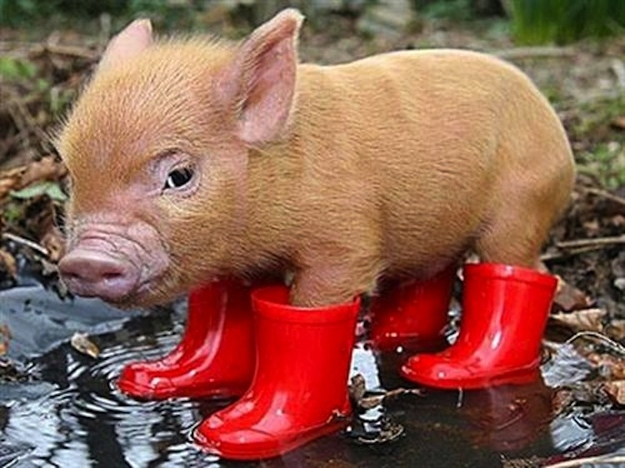
\includegraphics[width=0.8\textwidth]{graphics/raster/pig.jpg}
        \caption[Ferkel]{Ein Ferkel mit roten Gummistiefeln}
        \label{fig:ferkel}
\end{figure}